\documentclass[12pt]{extarticle}
\usepackage[utf8]{inputenc}
\usepackage{amsmath}
\usepackage{graphicx}
\usepackage{parskip}

\title{Scaling Law}
\date{\today}

\begin{document}



\section{Scaling Law}

\subsection{Isobaric Core Radius---Version-1}

Goal: Equivalent heat deposition for 2D and 3D


$R_{\mathrm{planet}}$ = Radius of the planet

$R_{\mathrm{core}}$ = Radius of the core

$r_{\mathrm{sphere}}$ = Radius of isobaric core = $\sqrt[3]{3} \times r_{\mathrm{imp}}$ 

$r_{\mathrm{circle}} = ?$


\begin{align*}
   &\frac{A_{\mathrm{ic}}}{A_{\mathrm{planet}}-A_{\mathrm{core}}} = \frac{V_{\mathrm{ic}}}{V_{\mathrm{planet}}-V_{\mathrm{core}}} &  \\
   %
   &\frac{\pi r_{\mathrm{circle}}^2}{\pi (R_{\mathrm{planet}}^2-R_{\mathrm{core}}^2)}  =  \frac {\frac{4}{3} \pi r_{\mathrm{sphere}}^3 } {\frac{4}{3} \pi (R_{\mathrm{planet}}^3-R_{\mathrm{core}}^3) }& \\
   %
   &r_{\mathrm{circle}} = \sqrt{r_{\mathrm{sphere}}^3 \left(\frac{R_{\mathrm{planet}}^2 - R_{\mathrm{core}}^2}{R_{\mathrm{planet}}^3 - R_{\mathrm{core}}^3}\right)}& \\
   %
   &r_{\mathrm{circle}} = \sqrt{\left({\sqrt[3]{3} \times r_{\mathrm{imp}}}\right)^3 \left(\frac{R_{\mathrm{planet}}^2 - R_{\mathrm{core}}^2}{R_{\mathrm{planet}}^3 - R_{\mathrm{core}}^3}\right)} & \\
   %
   &r_{\mathrm{circle}} = r_{\mathrm{imp}}^{\frac{3}{2}} \times \sqrt{3 \left(\frac{R_{\mathrm{planet}}^2 - R_{\mathrm{core}}^2}{R_{\mathrm{planet}}^3 - R_{\mathrm{core}}^3}\right)}& \\
   &r_{\mathrm{circle}} = r_{\mathrm{imp}}^{\frac{3}{2}} \times 0.00064967601& \\
\end{align*}

\clearpage

Now, scale $r_{\mathrm{imp}}$:

\begin{align*}
   &r_{\mathrm{circle}} = r_{\mathrm{imp}}^{\frac{3}{2}} \times 0.00064967601& \\
   %
   &\sqrt[3]{3} \times r_{\mathrm{imp}}' = r_{\mathrm{imp}}^{\frac{3}{2}} \times 0.00064967601& \\
   %
   &r_{\mathrm{imp}}' = r_{\mathrm{imp}}^{\frac{3}{2}} \times 0.00045046019& \\
\end{align*}

\vspace{1cm}

\subsection{Isobaric Core Radius---Version-2}

The version---1 scaling law considered the whole volume (area for 2D) of the isocore. But the whole isocore is not inside the planet. In StagYY, the distance between the centre of the planet and the centre of the isocore, $d = R-r/2$. In 2D, that looks like the following figure.

\begin{figure}[th]
    \centering
    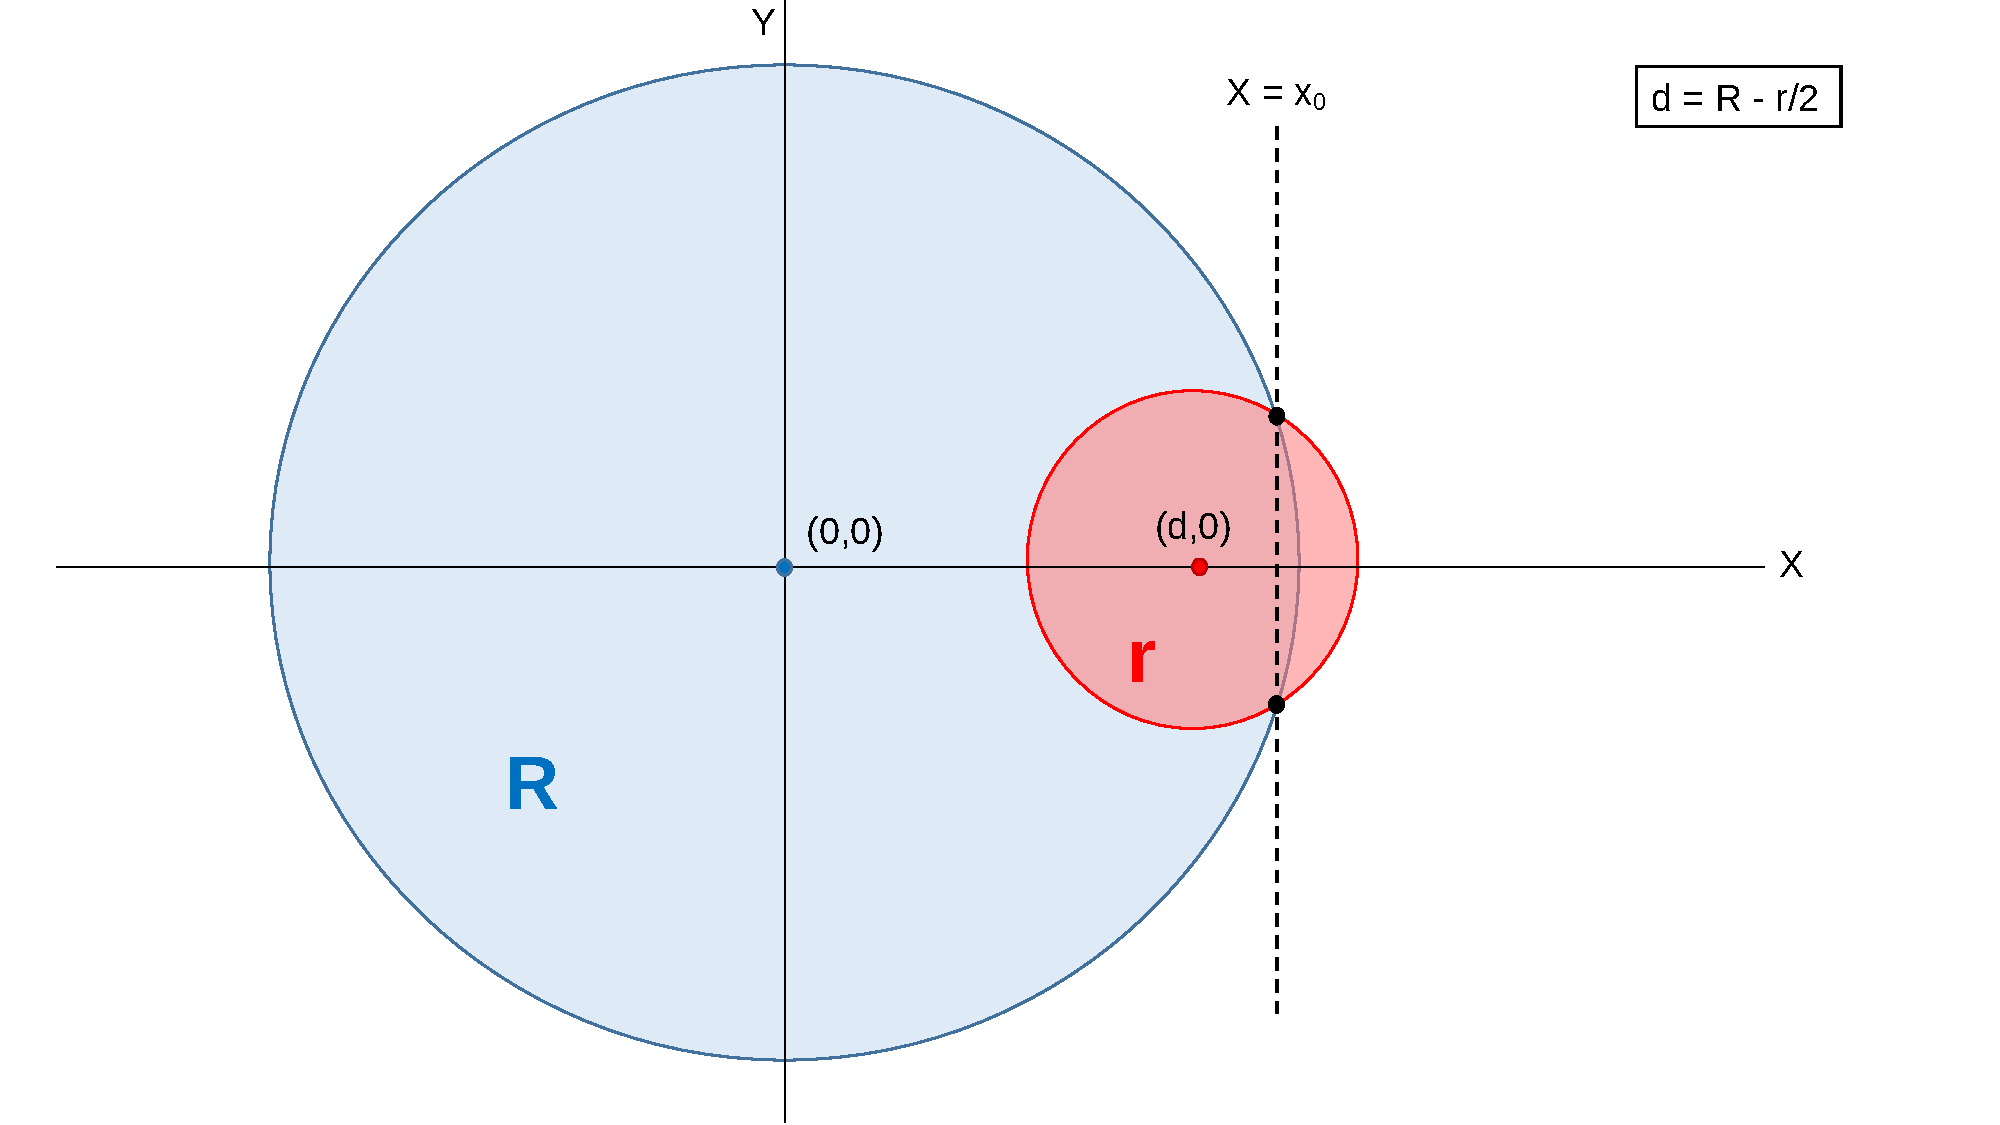
\includegraphics[width=0.98\textwidth]{Presentation1.pdf}
    %\caption{\footnotesize\textbf{Comparison between the composite model and the two models: }$R_{\mathrm{min}} = 50$ km and $R_{\mathrm{max}}=2443$ km  }
    \label{fig:2D}
\end{figure}

We need to exclude the volume (area for 2D) outside the planet. So we need to integrate the volume (area for 2D) upto R. The whole integration is divided into two parts.

(1) Integrate the volume (area for 2D) "under" the "curve" of the isocore from $d = R-r/2$ to $x_0$

(2) Integrate the volume (area for 2D) "under" the "curve" of the planet from $x_0$ to $R$

Then add them.









\subsubsection{Area of the isocore in 2D}

The planet of radius $R$ is at $(0,0)$. The isocore of radius $r$ is at $(d,0)$ where $d = R-r/2$. The isocore intersects the planet at $X=x_0$. First, we need to figure out $x_0$ as this is the limit for the integrations.

The equation of the isocore:

    \begin{align*} 
       (x-d)^2 + y^2 = r^2 \\
       y^2 = r^2 - (x-d)^2 \\
    \end{align*}

The equation of the planet:

    \begin{align*} 
       x^2 + y^2 = R^2 \\
       y^2 = R^2 - x^2 \\
    \end{align*}

From this we can write: 

    \begin{align*} 
      &R^2 - x^2 = r^2 - (x-d)^2 \\
      &x = x_0 = \frac{R^2 - r^2 + d^2}{2d} \tag{1} \\
    \end{align*}

\clearpage

\textbf{Part---1:} Area "under" the isocore curve (A$_1$)

Isocore equation:

    \begin{align*} 
       &y^2 = r^2 - (x-d)^2 \\
       &y = \sqrt{r^2 - (x-d)^2}
    \end{align*}

So, the total area "under" the isocore curve,

    \begin{align*} 
      A_1 = 2 \int_{d-r}^{x_0} \sqrt{r^2 - (x-d)^2} \,dx 
    \end{align*}

Put $x-d = u$ or $dx = du$

When $x = d-r$, $u = x-d = (d-r)-d = -r$

When $x = x_0$, $u = x_0 - d = u_0$

So the integration becomes:

    \begin{align*} 
      A_1 &= 2 \int_{-r}^{u_0} \sqrt{r^2 - u^2} \,du \\
      &= 2\left[  \frac{u \sqrt{r^2 - u^2}}{2} + \frac{r^2}{2} \sin^{-1}{ \left(  \frac{u}{r}  \right)  }   \right]_{-r}^{u_0} \\
      &= 2\left[\left\{  \frac{u_0 \sqrt{r^2 - {u_0}^2}}{2} + \frac{r^2}{2} \sin^{-1}{\left(\frac{u_0}{r}\right)}   \right\} - \left\{ \frac{r^2}{2} \sin^{-1} (-1)  \right\}   \right] \\
      &= u_0 \sqrt{r^2 - {u_0}^2} + r^2 \sin^{-1} \left(   \frac{u_0}{r}   \right) + \frac{r^2 \pi}{2} \tag{2}
    \end{align*}


\textbf{Part---2:} Area "under" the planet curve (A$_2$)


Planet equation:

    \begin{align*} 
       &y^2 = R^2 - x^2 \\
       &y = \sqrt{R^2 - x^2} \\
    \end{align*}

So, the total area "under" the planet curve,

    \begin{align*} 
      A_2 &= 2 \int_{x_0}^{R} \sqrt{R^2 - x^2} \,dx \\
      &= 2 \left[   \frac{x \sqrt{R^2 - x^2}}{2} + \frac{R^2}{2} \sin^{-1}{ \left(\frac{x}{R} \right) }  \right]_{x_0}^R \\
      &= 2 \left[  \left\{  \frac{R^2}{2} \sin^{-1}{(1)}  \right\} - \left\{ \frac{x_0 \sqrt{R^2-{x_0}^2}}{2} + \frac{R^2}{2} \sin^{-1}{\left(  \frac{x_0}{R} \right)} \right\}  \right] \\
      &= \frac{R^2 \pi}{2} - x_0 \sqrt{R^2 - {x_0}^2} - R^2 \sin^{-1}{\left( \frac{x_0}{R} \right)} \tag{3}
    \end{align*}

So, total area of the isocore:

    \begin{align*} 
     A &= A_1 + A_2 \\
     &= \left\{ u_0 \sqrt{r^2 - {u_0}^2} + r^2 \sin^{-1} \left(   \frac{u_0}{r}   \right) + \frac{r^2 \pi}{2} \right\} + 
        \left\{  \frac{R^2 \pi}{2} - x_0 \sqrt{R^2 - {x_0}^2} - R^2 \sin^{-1}{\left( \frac{x_0}{R} \right)}  \right\}
    \end{align*}



\vspace{0.5cm}










\subsubsection{Volume of the isocore in 3D}

$x_0$ and $d$ remain same. 

The planet of radius $R$ is at $(0,0,0)$. The isocore of radius $r$ is at $(d,0,0)$. The isocore intersects the planet at $X=x_0$.


\textbf{Part---1:} Volume inside the isocore curve (V$_1$)

At a given $X$, a $YZ$ plane intersects the isocore, creating a circle. The radius of the circle is a function of distance from the centre of the planet.

The equation of isocore sphere:

    \begin{align*} 
        (x-d)^2 + y^2 + z^2 = r^2 \\
        y^2 + z^2 = r^2 - (x-d)^2 \tag{4}
    \end{align*}
The RHS of equation $(4)$ is the radius$^2$ of said circle.

So, the area of said circle

    \begin{align*} 
        = \pi \left\{r^2 - (x-d)^2\right\}
    \end{align*}


The total volume inside the isocore:
        
    \begin{align*} 
        V_1 &= \int_{d-r}^{x_0}  \pi \left\{r^2 - (x-d)^2\right\}  \,dx \\
        &= \pi \int_{d-r}^{x_0} (r^2 - x^2 + 2xd - d^2) \,dx \\
        &= \pi \left[  r^2 x - \frac{x^3}{3} + x^2d -d^2x   \right]_{d-r}^{x_0} \\
        &= \pi \left[ \left\{ r^2 x_0 - \frac{{x_0}^3}{3} + {x_0}^2d -d^2x_0 \right\} -   \left\{ r^2 (d-r) - \frac{(d-r)^3}{3} + (d-r)^2 d - d^2 (d-r) \right\}   \right]
    \end{align*}


\textbf{Part---2:} Volume inside the planet curve (V$_2$)

The equation of the planet sphere:

    \begin{align*} 
        x^2 + y^2 + z^2 = R^2 \\
        y^2 + z^2 = R^2 - x^2 \\
    \end{align*}

Area of the intersection circle:

    \begin{align*} 
        \pi (R^2 - x^2)
    \end{align*}

So, total volume inside the planet sphere:

    \begin{align*} 
       V_2 &= \int_{x_0}^{R} \pi (R^2 - x^2) \,dx  \\
       &= \pi \left[  R^2 x - \frac{x^3}{3}  \right]_{x_0}^R \\
       &= \pi (R^3 - \frac{R^3}{3} - R^2 x_0 + \frac{{x_0}^3}{3}) \\
    \end{align*}

So the total volume of the isocore

    \begin{align*} 
       V &= V_1 + V_2 \\
       &= \pi \left[ \left\{ r^2 x_0 - \frac{{x_0}^3}{3} + {x_0}^2d -d^2x_0 \right\} -   \left\{ r^2 (d-r) - \frac{(d-r)^3}{3} + (d-r)^2 d - d^2 (d-r) \right\}   \right] \\
       &+ \pi (R^3 - \frac{R^3}{3} - R^2 x_0 + \frac{{x_0}^3}{3}) \\
    \end{align*}

\end{document}








